\subsection{Changes Over Epochs}
To explore the model behavior over the training process, we manually select the RNN model trained under epoch numbers of 5, 40, 120, and 200. Fig.~\ref{fig:evolution_epochs} shows the projections and top five most important features at different epochs.

In the Projection View (Fig.~\ref{fig:evolution_epochs}A), we choose $PM_{2.5}$ as the target feature and use a sequential color schema to indicate the predicted value where a darker color indicates a higher $PM_{2.5}$. 
At early stages ($5^{th}$ and $40^{th}$ epochs), we find that the points with a deep color are distributed uniformly in the projection and are mixed together with the points with a light color. 
This indicates that the cluster gradients are not able to present the distribution of the target feature yet.
When trained after more epochs, the dark points become more concentrated. 

In addition, the Feature Importance View (Fig.~\ref{fig:evolution_epochs}B) shows that the magnitude of the gradient starts from a small value and then keeps increasing in the training process. 
We also find that in the $5^{th}$ and $40^{th}$ epochs, the top five important features are $\color{PM25Color}{PM_{2.5}}$ and $\color{PM10Color}{PM_{10}}$ while in the $120^{th}$ epoch, the feature of wind speed is also ranked in the top five most important features. 
In the $200^{th}$ epoch, more features related to wind speed are listed in the top five features.
Another finding is that in the $5^{th}$ epoch, we observe that only the features from the last time steps are considered important while the models at the $40^{th}$, $120^{th}$, and $200^{th}$ epochs leverage more timestamps in the forecast.  
The domain experts indicate that the $PM_{2.5}$ and $PM_{10}$ at nearby locations are the most intuitive features to forecast $PM_{2.5}$ ($PM_{10}$ and $PM_{2.5}$ are always highly correlated).
Moreover, the last time step is very important because it is the closest one to the final prediction. 
Based on these observations, we infer that the features that are directly related with the targeted air pollutant are considered important in the early stage of the training process.
After more epochs, the model starts to learn other features that may indirectly influence the forecast, such as the \textit{\color{WINDColor}{Wind Speed}} and other pollutants ($\color{SO2Color}{SO_2}$ or $\color{NO2Color}{NO_2}$) (shown as \ref{fig:evolution_epochs}1B, 20$^{th}$,200$^{th}$ epochs). 

We discussed the reason that $SO_2$ becomes important later in training with the domain experts. 
% They explained that the sulfur oxides ($SO_x$) react with other compounds in the air and form tiny particles which contribute to the particulate matter. 
A "Report on the Environment" from the EPA (United States Environmental Protection Agency) indicates that ``SO2 emissions are an important environmental issue because they are a major precursor to ambient $PM_{2.5}$ concentrations."\ref{}
Moreover, the domain experts explain that the wind speed is important for several reasons: 1) the air pollutants will  be blown away if the wind speed is high; 2) since the north and west of the target location have more factories which are the major source of air pollutants, the appropriate wind speed and direction will bring the air pollutants to Hong Kong.
Moreover, the data also show different patterns in the Cluster View during the training process. 
For example, as shown in Fig.\ref{fig:evolution_epochs}B, we found that in the $5^{th}$ epoch almost all three types of features: \textit{\color{SLPColor}{Sealevel Pressure}}, \textit{\color{DPColor}{Dew-point}} and  \textit{\color{SPColor}{Station Pressure}} are grouped into one cluster. 
After the $40^{th}$ epoch, we notice that this cluster is split into two clusters.
With these observations, we derive the conclusion that the model gradually learns the high-level knowledge in the training process.

\begin{figure}[t]
	\centering
	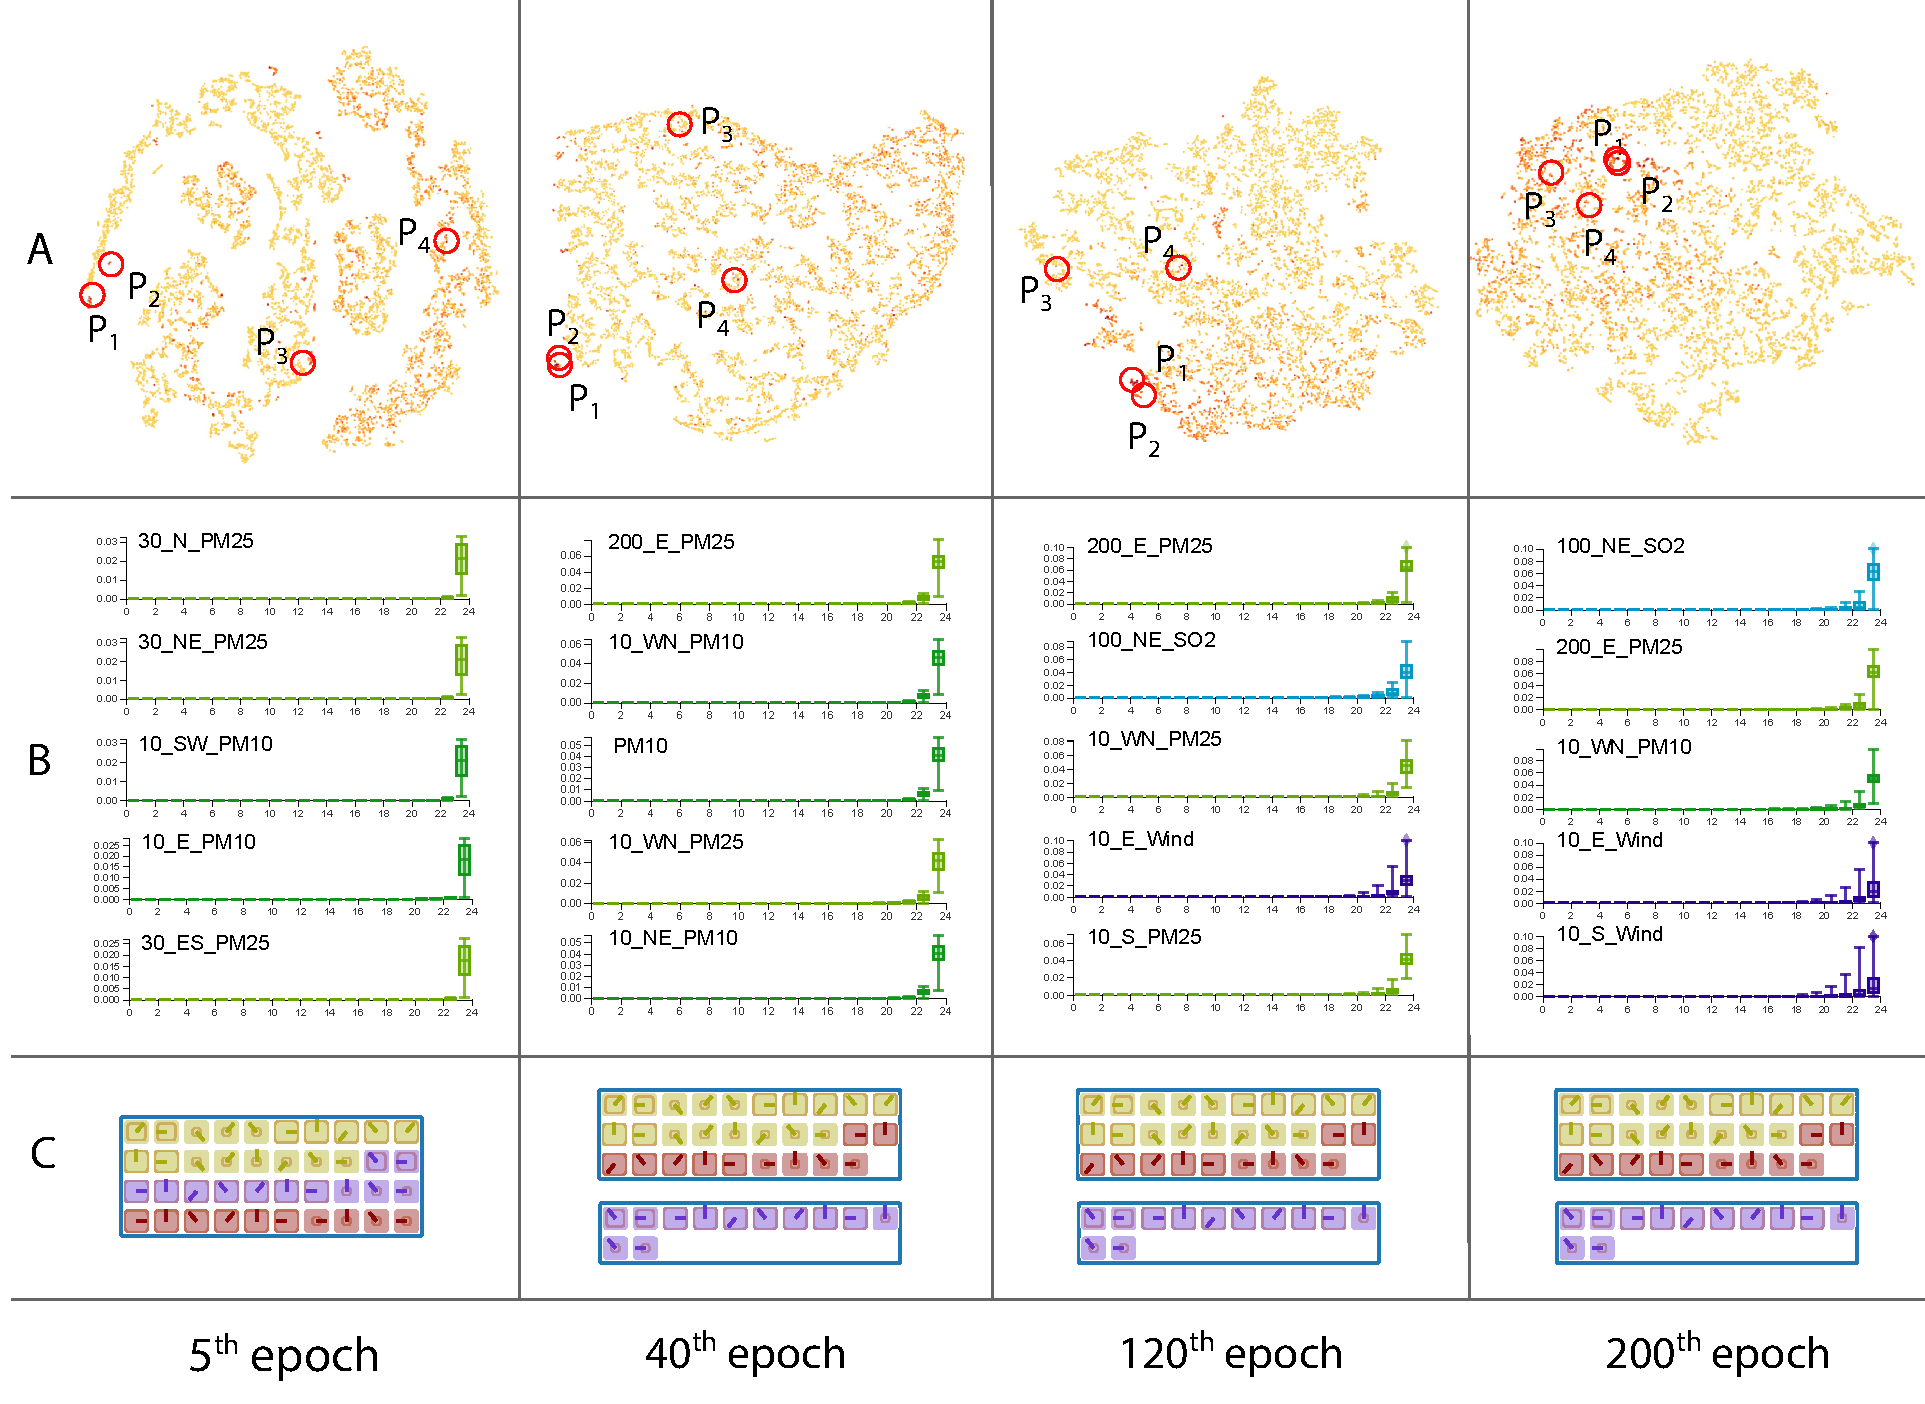
\includegraphics[width=0.45\textwidth]{pictures/Evaluation/evolution_epochs.pdf}
	\vspace{-3mm}
	\caption{\UC{The model behavior over the learning process. A, B and C show the Projection View, top five important features and feature clusters at the corresponding epochs.}
% 	A: Projection Views shows the high-pollutant points gradually gathered during the training process; B: the top five important features at the corresponding epochs; C: the feature cluster change at each epoch.
	}
	\label{fig:evolution_epochs}
	\vspace{-4mm}
\end{figure}

